% https://tex.stackexchange.com/q/232816/173708
\documentclass[tikz,border=9]{standalone}
\usetikzlibrary{mindmap}
\usepackage{xspace}
\definecolor{joli}{RGB}{225,95,0}
\definecolor{JOLI}{RGB}{225,95,0}
\newcommand\etoc{\textcolor{joli}{\ttfamily\bfseries etoc}\xspace}
\DeclareRobustCommand\csa[1]{{\ttfamily\hyphenchar\font45 \char`\\ #1}}

\newcount\tikznumberofcurrentgrandchild

\def\tikzmycustomgrowth {%
  \pgftransformreset
  \ifnum\tikztreelevel=1
    \pgftransformrotate {(\pgfkeysvalueof{/tikz/sibling angle})*(\tikznumberofcurrentchild-1)}%
  \fi
  \ifnum\tikztreelevel=2
    \pgftransformrotate {(\pgfkeysvalueof{/tikz/sibling angle})*(\tikznumberofcurrentgrandchild-4)}%
    \global\advance\tikznumberofcurrentgrandchild by 1
 \fi
 \pgftransformxshift {\the\tikzleveldistance}%
}
\tikzset{
    branch color/.style={
        concept color=#1!white,
        every child/.append style={concept color=#1!white!30!white},
    }
}

\begin{document}
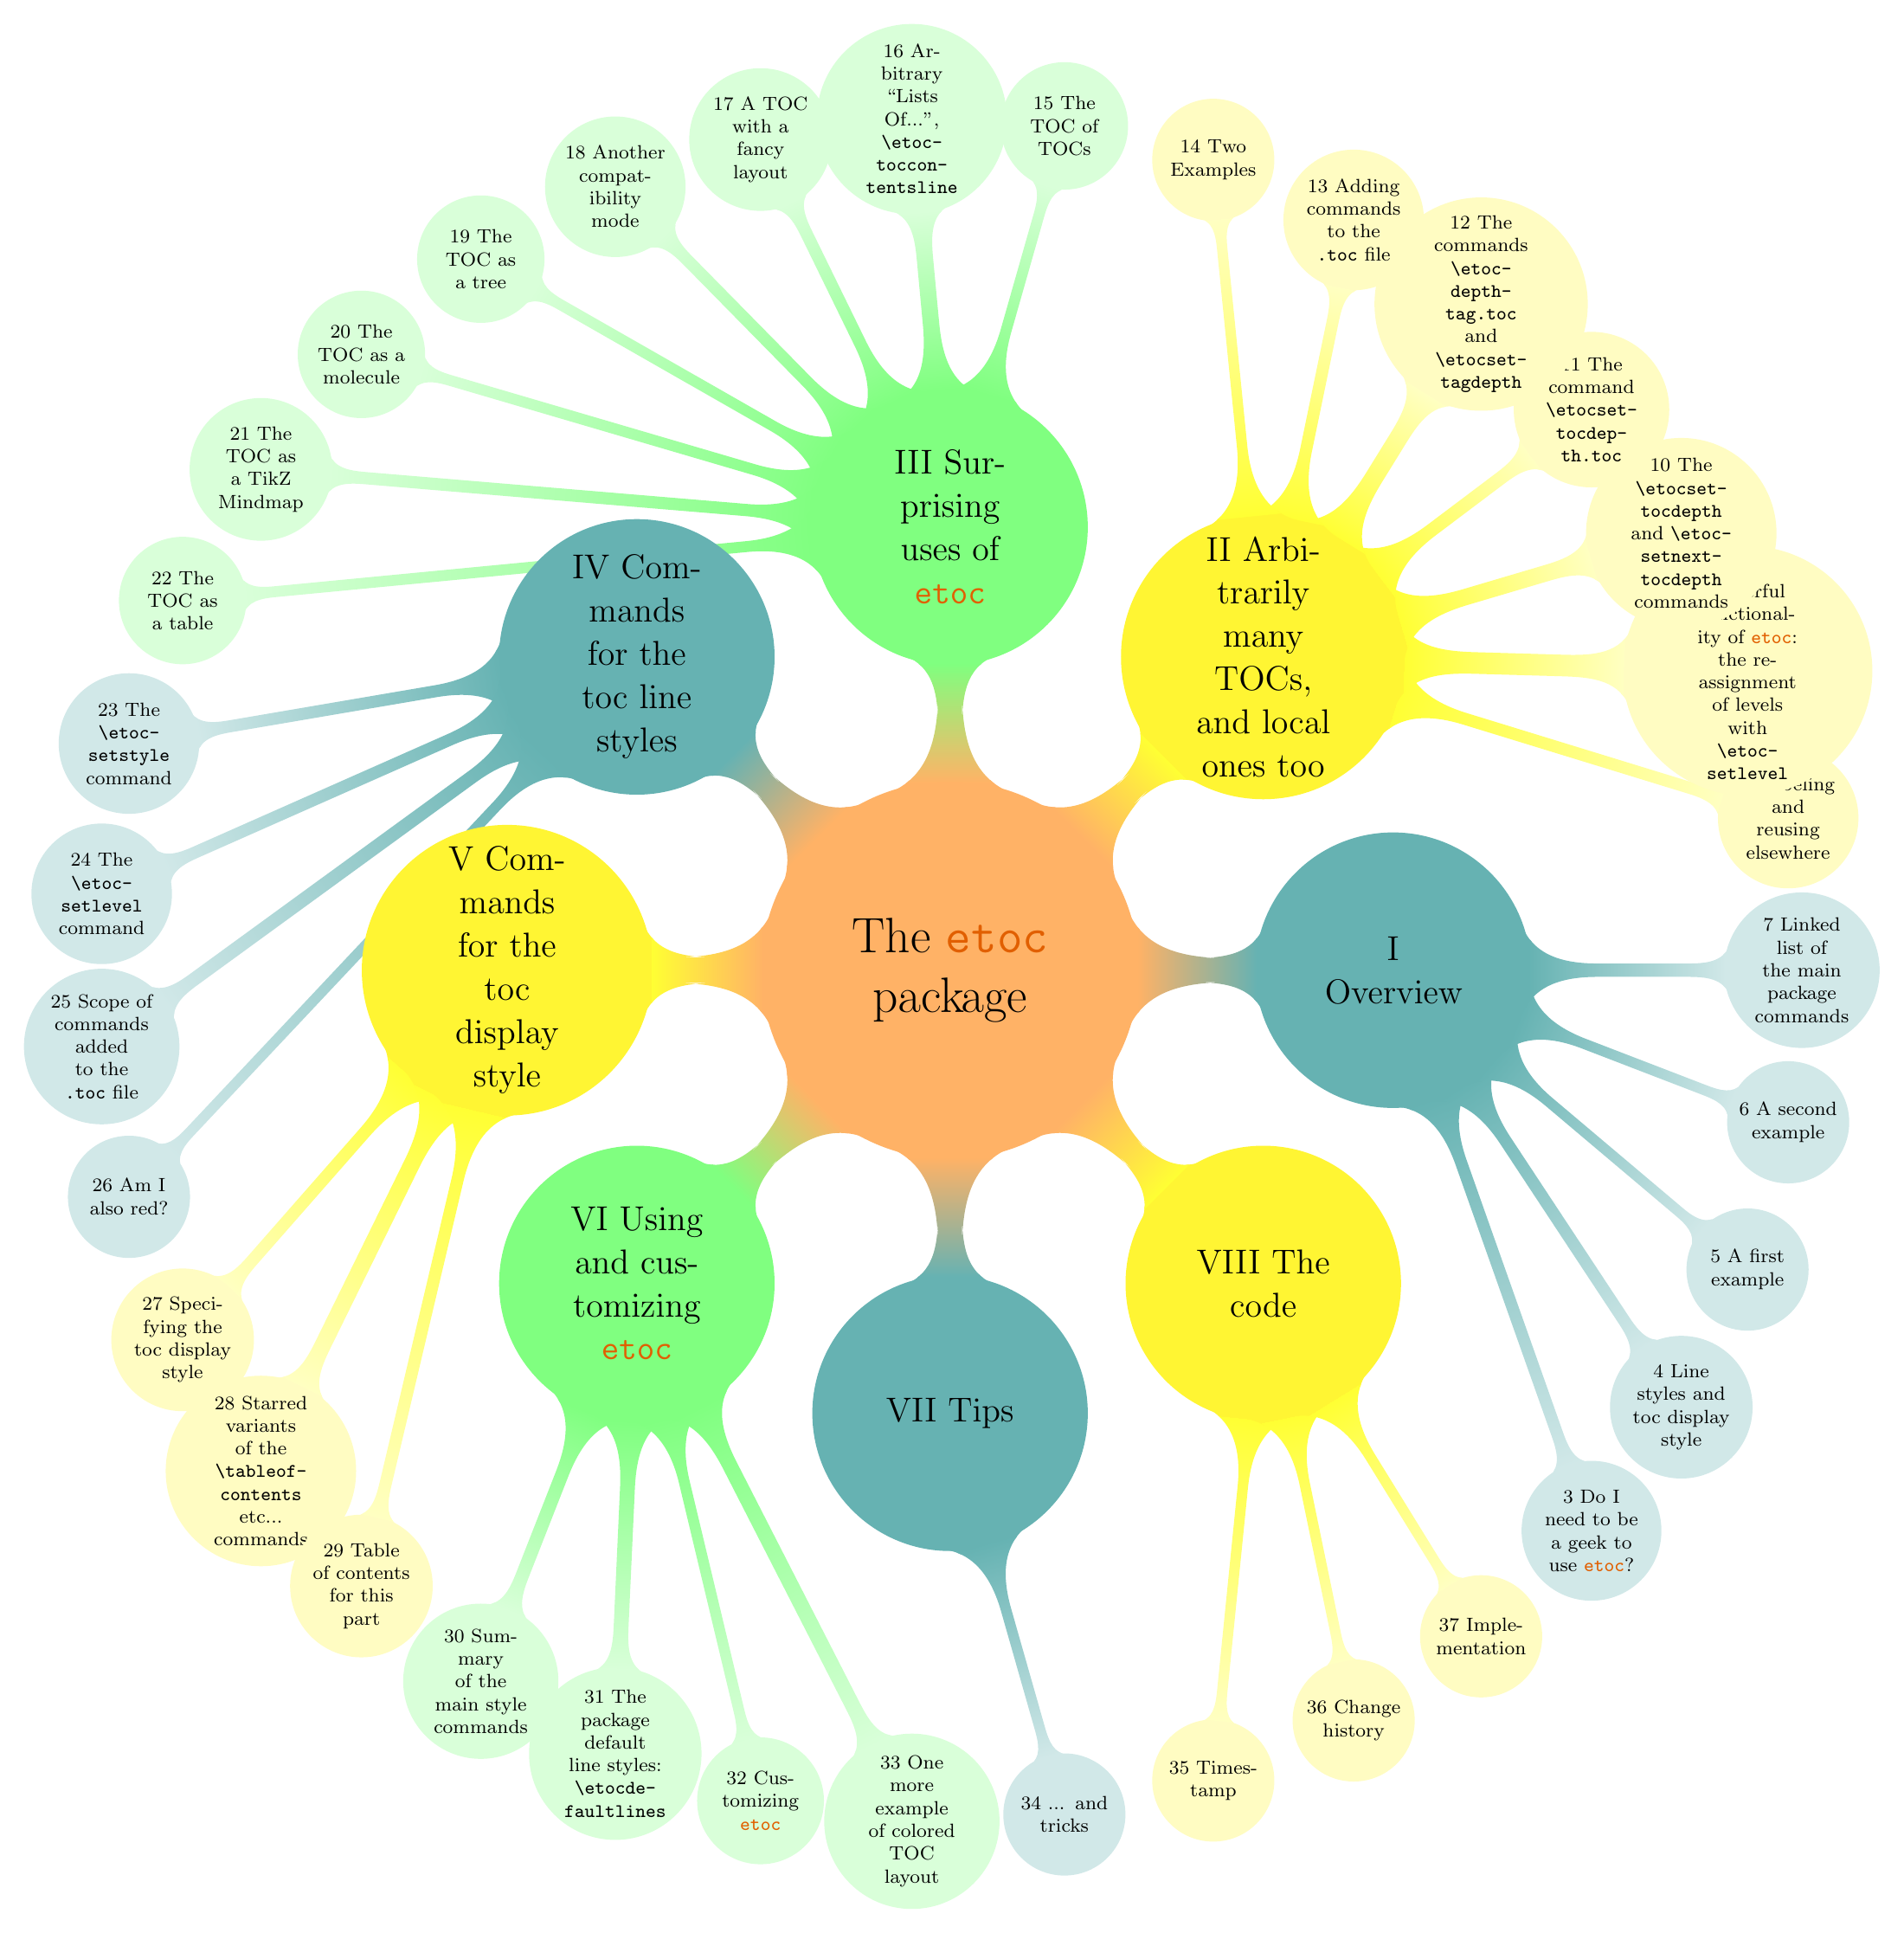
\begin{tikzpicture}
  [
    mindmap,
    growth function=\tikzmycustomgrowth,
    nodes={concept},
    concept color=orange!60,
    root concept/.append style={font=\huge, minimum size=5.5cm},
    level 1/.append style={level distance=6.5cm, sibling angle=360/8},
    level 1 concept/.append style={font=\Large,minimum size=4cm},
    level 2/.append style={level distance=12.5cm, sibling angle=360/35},
    % distance par rapport au CENTRE ! (avec le code tel qu'en ce moment)
  ]
  \tikznumberofcurrentgrandchild=0
  \node [root concept]{The \etoc package} 
  child [branch color=teal!60]{node {I Overview} 
  child {node {3 Do I need to be a geek to use {\color {joli}\ttfamily \bfseries etoc}\xspace ?}} 
  child {node {4 Line styles and toc display style}} 
  child {node {5 A first example}} 
  child {node {6 A second example}} 
  child {node {7 Linked list of the main package commands}}} 
  child [branch color=yellow!80]{node {II Arbitrarily many TOCs, and local ones too} 
  child {node {8 Labeling and reusing elsewhere}} 
  child {node {9 A powerful functionality of {\color {joli}\ttfamily \bfseries etoc}\xspace : the re-assignment of levels with \csa {etocsetlevel}}} 
  child {node {10 The \csa {etoc\discretionary {-}{}{}set\discretionary {-}{}{}toc\discretionary {-}{}{}depth} and \csa {etoc\discretionary {-}{}{}set\discretionary {-}{}{}next\discretionary {-}{}{}toc\discretionary {-}{}{}depth} commands}} 
  child {node {11 The command \csa {etoc\discretionary {-}{}{}set\discretionary {-}{}{}toc\discretionary {-}{}{}dep\discretionary {-}{}{}th.toc}}} 
  child {node {12 The commands \csa {etoc\discretionary {-}{}{}depth\discretionary {-}{}{}tag.toc} and \csa {etocsettagdepth}}} 
  child {node {13 Adding commands to the \texttt {.toc} file}} 
  child {node {14 Two Examples}}} 
  child [branch color=green!50]{node {III Surprising uses of {\color {joli}\ttfamily \bfseries etoc}\xspace } 
  child {node {15 The TOC of TOCs}} 
  child {node {16 Arbitrary ``Lists Of...'', \csa {etoctoccontentsline}}} 
  child {node {17 A TOC with a fancy layout}} 
  child {node {18 Another compatibility mode}} 
  child {node {19 The TOC as a tree}} 
  child {node {20 The TOC as a molecule}} 
  child {node {21 The TOC as a TikZ Mindmap}} 
  child {node {22 The TOC as a table}}} 
  child [branch color=teal!60]{node {IV Commands for the toc line styles} 
  child {node {23 The \csa {etocsetstyle} command}} 
  child {node {24 The \csa {etocsetlevel} command}} 
  child {node {25 Scope of commands added to the \texttt {.toc} file}} 
  child {node {26 Am I also red?}}} 
  child [branch color=yellow!80]{node {V Commands for the toc display style} 
  child {node {27 Specifying the toc display style}} 
  child {node {28 Starred variants of the \csa {tableofcontents} etc... commands}} 
  child {node {29 Table of contents for this part}}} 
  child [branch color=green!50]{node {VI Using and customizing {\color {joli}\ttfamily \bfseries etoc}\xspace } 
  child {node {30 Summary of the main style commands}} 
  child {node {31 The package default line styles: \csa {etocdefaultlines}}} 
  child {node {32 Customizing {\color {joli}\ttfamily \bfseries etoc}\xspace }} 
  child {node {33 One more example of colored TOC layout}}} 
  child [branch color=teal!60]{node {VII Tips} 
  child {node {34 ... and tricks}}} 
  child [branch color=yellow!80]{node {VIII The code} 
  child {node {35 Timestamp}} 
  child {node {36 Change history}} 
  child {node {37 Implementation}}} ;
\end{tikzpicture}
\end{document}